\chapter{Server E2E tests}\label{ch:apx-server-e2e-tests}

\section{Server E2E test file}\label{sec:full-server-e2e-test-file}

\codeFromFile{ts}{../apps/server-e2e/src/app.e2e-spec.ts}{Sever E2E test file}{Sever E2E test file}{lst:apx-full-server-e2e-test-file}

\section{Server E2E test results}\label{sec:full-server-e2e-test-results}

\begin{figure}[H]
    \centering
    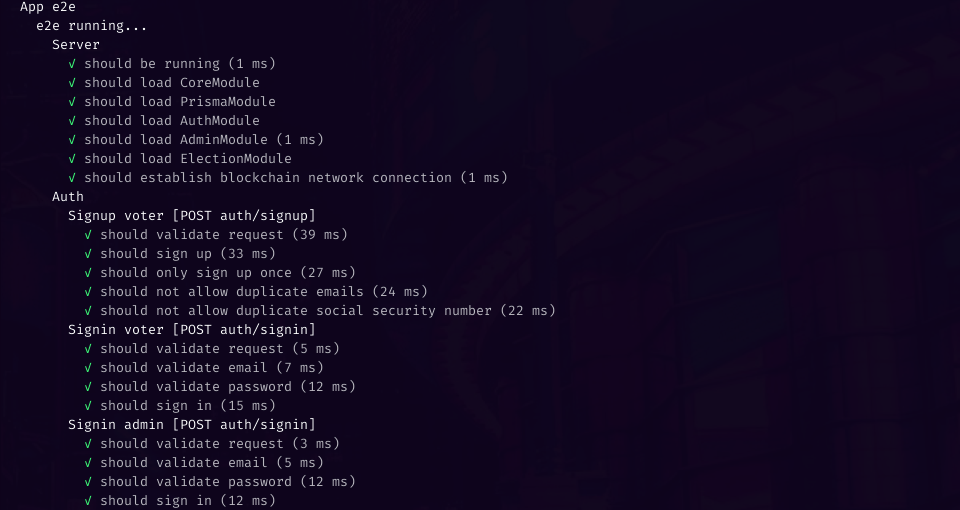
\includegraphics[width=\textwidth-50px]{boehm-e2e-tests1}
    \caption[Server E2E test results of initialization and auth module]{Server E2E test results of initialization and auth module. Screenshot taken by author}
    \label{fig:apx-e2e-tests-1}
\end{figure}

\begin{figure}[H]
    \centering
    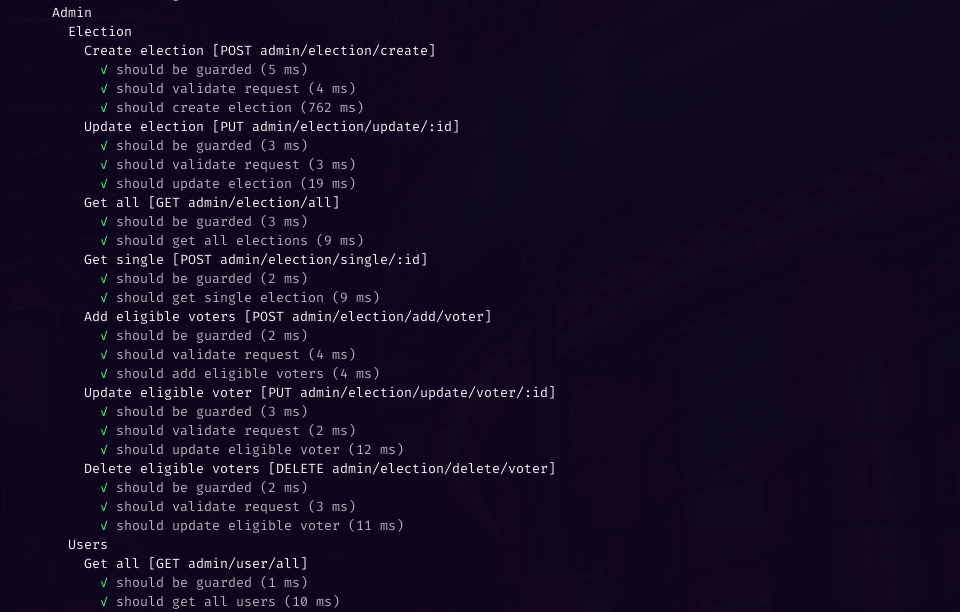
\includegraphics[width=\textwidth-50px]{boehm-e2e-tests2}
    \caption[Server E2E test results of admin module]{Server E2E test results of admin module. Screenshot taken by author}
    \label{fig:apx-e2e-tests-2}
\end{figure}

\begin{figure}[H]
    \centering
    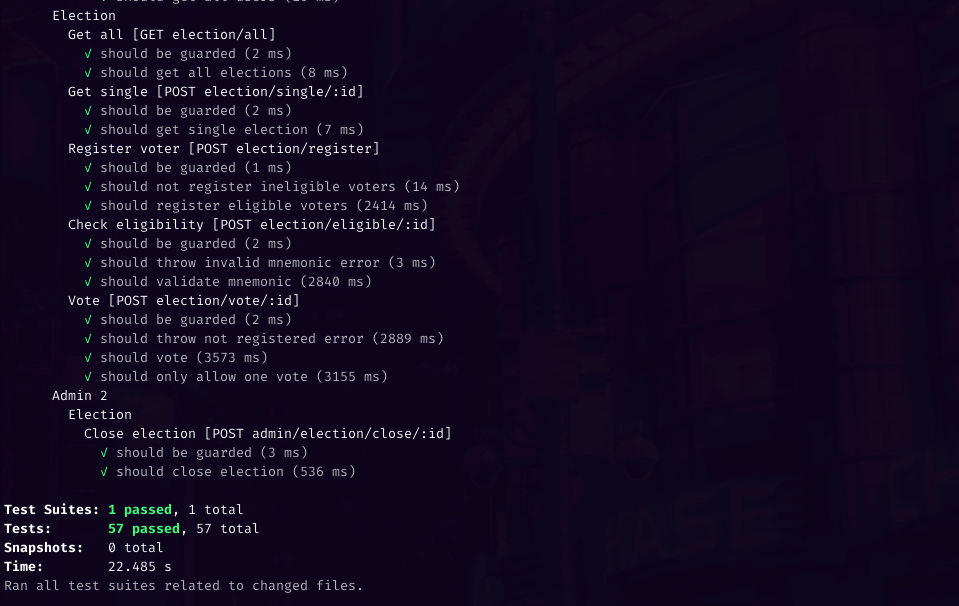
\includegraphics[width=\textwidth-50px]{boehm-e2e-tests3}
    \caption[Server E2E test results of election module]{Server E2E test results of election module. Screenshot taken by author}
    \label{fig:apx-e2e-tests-3}
\end{figure}

This section provides a full overview of all \gls{E2E} test results that were run against our backend application:

\begin{enumerate}
    \item Results of initialization and auth module tests (see~\cref{fig:apx-e2e-tests-1})
    \item Results of admin module tests (see~\cref{fig:apx-e2e-tests-2})
    \item Results of election module tests (see~\cref{fig:apx-e2e-tests-3})
\end{enumerate}

